\chapter{Basics of Terrain Rendering}
\section{Terrain Data Representation}
\subsection{Heightmaps}
One way of representing terrains is using \textit{heightmaps}.
A heightmap is a $n\times n$-grid that contains 
the height value $y$ for each $(x,z)$-position\footnote{We always denote $y$ for the up direction except if explicitly stated otherwise.}.
Positions are always spaced evenly in a grid-like manner,
but the distance between any two neighboring positions is variable.

The main advantage of heightmaps is that they allow for very simple storage and manipulation of height data, e.g. in form of images,
where low color values represent low areas of terrain and vice versa for
high color values. For a grayscale image, up to 256 height values can be used and for an RGB image,
more than 16 million height values are supported.
Looking up a height value for a given $(x,z)$-position is easy as well,
which consists of a simple lookup at the given position in the image.
Figure~\ref{fig:dom} shows a $2000 \times 2000$ heightmap of the mountain Dom in Valais, Switzerland.
\begin{figure}[H]
  \centering
  
\includegraphics[width=0.4\textwidth]{dom}
  \caption{$2000 \times 2000$ heightmap of the mountain Dom in Valais, Switzerland retrieved from SwissTopo \cite{alti3d}.}\label{fig:dom}
\end{figure}

\subsection{Triangulated Irregular Networks}
An alternative to the heightmap is the \textit{triangulated irregular network (TIN)} data structure.
A TIN consists of a collection of 3D vertices, where 
the arrangement of vertices can be irregular. Figure~\ref{fig:tin-example} shows 
an example of a TIN.
\begin{figure}[H]
  \centering
  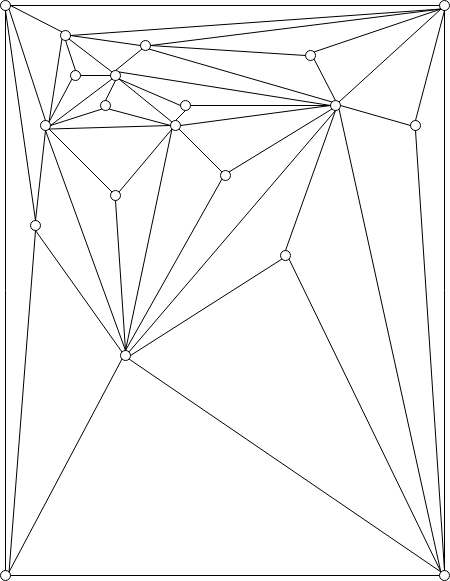
\includegraphics[width=0.52\textwidth]{tin-example}
  \caption{Example of a TIN. Note that the left area represents a terrain area with many changes 
  (e.g. mountains, hills, etc.), and the right area represents an area with few changes (e.g. flat areas).}\label{fig:tin-example}
\end{figure}

The main advantage of TINs is that fewer polygons need to be used for 
e.g. smooth terrain areas. Another advantage is that
special terrain features can be modelled 
which are usually difficult to model with heightmaps, such as overhangs, cliffs and caves, 
The disadvantage of TINs, however, is that the full $(x,y,z)$ coordinates need to be stored,
whereas with heightmaps, only the height value $y$ needs to be stored.

\section{Bintrees and Quadtrees}
\textit{Binary triangle trees (bintrees)} and \textit{quadtrees} are 
recursive data structures based on triangles and quads respectively.
A bintree consists of up to two child triangles, both of which in turn also consist of up to two child triangles each, and so on.
Quadtrees are structured similarly, with a quad consisting of up to four child quads, and each child quad consisting
of up to four child quads, and so on.
Figure~\ref{fig:bintree-quadtree-example} shows an example of a bintree and a quadtree.

\begin{figure}[H]
  \centering
  \subfloat[\centering]{{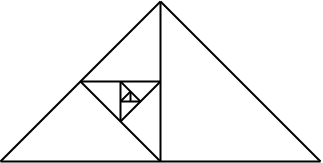
\includegraphics[width=0.43\textwidth]{bintree-example} }}
  \qquad
  \subfloat[\centering]{{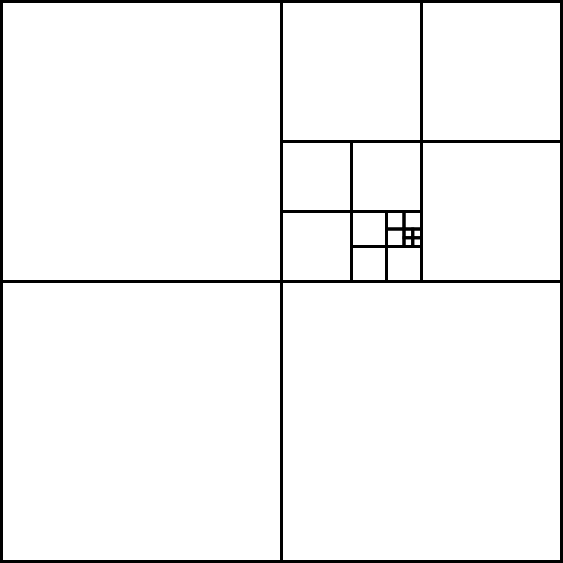
\includegraphics[width=0.33\textwidth]{quadtree-example.png} }}%
  \caption{Example of a bintree (a) and a quadtree (b).}\label{fig:bintree-quadtree-example}
\end{figure}

The main advantage of bintrees and quadtrees is that 
LOD can be modelled very naturally with them.
Bintree/quadtree sections with few children correspond to a low LOD and 
vice versa for bintree/quadtree sections with many children.

\section{Potential Problems During Terrain Rendering}
While terrain LOD algorithms dramatically improve the performance of terrain rendering, 
there are certain faults that can occur during rendering. 

\subsection{Cracks}
Cracks and holes in terrains can appear when a higher LOD terrain section is bordered 
by a lower LOD terrain section. The main problem is that when a vertex $v_{\text{high}}$ of a higher LOD terrain section lies on the edge $e_{\text{low}}$
of a lower LOD terrain section and the $y$ coordinate of $v_{\text{high}}$ is greater or less than the 
height of $e_{\text{low}}$ at that point, the difference in height causes the crack to appear, as shown in figure~\ref{fig:crack-example}.
\begin{figure}[H]
  \centering
  \subfloat[\centering The crack is caused by the height difference of $v_{\text{high}}$ and $e_{\text{low}}$.]{{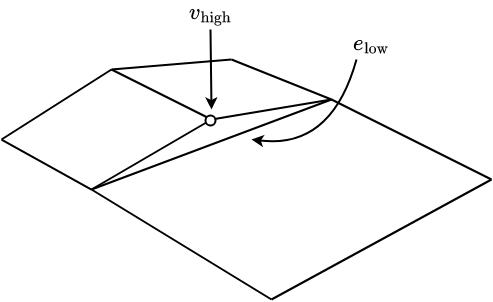
\includegraphics[width=0.5\textwidth]{crack-example} }}
  \qquad
  \subfloat[\centering The background color is set to red to highlight the cracks.]{{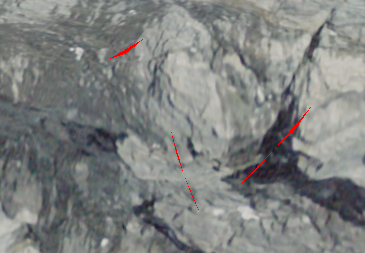
\includegraphics[width=0.4\textwidth]{cracks-terrain} }}%
  \caption{Illustration of a crack (a) and some examples of cracks in a real rendered terrain (b).}\label{fig:crack-example}
\end{figure}
Cracks can be solved by either of the following, depending on the capabilities of the LOD approach:
\begin{itemize}
  \item Removing the vertex in question, cuasing the higher and lower LOD meshes to be connected seamlessl (in figure~\ref{fig:crack-example} vertex $v_{\text{high}}$).
  \item Inserting an extra vertex at the border edge of the lower LOD mesh \cite[p.~194]{lodfor3dgraphics} (in figure~\ref{fig:crack-example} on top of vertex $v_{\text{high}}$). The disadvantage of this is that an extra vertex needs to get created.
  \item By force splitting the terrain mesh to get a more continuous mesh \cite[p.~193]{lodfor3dgraphics}. 
\end{itemize}

\subsection{Popping}
The phenomenon of \textit{popping} occurs when the camera is moving 
and the transition of the terrain's LOD level causes visual pops to appear.
Popping decreases the realism of the terrain and should be as minimal as possible.
Popping can be reduced by introducing \textit{vertex morphing} \cite{geomipmapping,geomclipmaps,cdlod}, 
i.e. by animating the transition of one LOD level to the next seamlessly through interpolation.